% https://de.overleaf.com/learn/latex/How_to_Write_a_Thesis_in_LaTeX_(Part_1)%3A_Basic_Structure
% https://en.wikibooks.org/wiki/LaTeX/Document_Structure
%\documentclass[11pt, twoside]{report}
\documentclass[11pt, a4paper]{report}
%\documentclass[a4paper,11pt]{scrartcl}
\usepackage{syntonly}
%\syntaxonly
\usepackage[utf8]{inputenc}
\usepackage[backend=biber]{biblatex}
\addbibresource{mybib.bib}
\usepackage{hyperref}
\usepackage{graphicx}
\usepackage{color}
\usepackage{framed}
\usepackage{subcaption}
\usepackage{float}
\graphicspath{ {images/} }
\usepackage{blindtext}
\usepackage{mathtools}
\usepackage{amssymb}
\usepackage{amsbsy}
\usepackage{amsfonts}
\usepackage{amsthm}
\usepackage{amsmath}
\usepackage{IEEEtrantools}
%\usepackage{showframe}
%\usepackage[a4paper, width=150mm, top=5mm, bottom=5mm]{geometry}
\usepackage[a4paper, width=150mm, top=25mm, bottom=25mm]{geometry}
\usepackage{fancyhdr}
%\setlength{\headheight}{12pt}
%\setlength{\headheight}{15.2pt}
%\pagestyle{empty}
%\pagestyle{myheadings}
%\pagestyle{headings}
%\pagestyle{plain}
\pagestyle{fancy}
\fancyhf{}
%\fancyhead[L]{\leftmark:}
%\fancyhead[L]{\chapter~\thechapter:}
%\fancyhead[L]{\thechapter}
\fancyhead[C]{\rightmark}
%\fancyhead[R]{\thesection}
\fancyfoot[C]{\thepage}

\setlength{\parskip}{1.0em}
\setlength{\parindent}{1em}

\usepackage{lipsum}

\theoremstyle{plain}
\newtheorem{theorem}{Theorem}[chapter]
\newtheorem{lemma}[theorem]{Lemma}

\theoremstyle{definition}
\newtheorem{mydef}{Definition}[chapter]

\theoremstyle{remark}
\newtheorem{remark}{Remark}[chapter]


%newcommands
\newcommand{\N}{\mathbb{N}}
\newcommand{\C}{\mathbb{C}}
\newcommand{\R}{\mathbb{R}}
%\newcommand{\Z}{\mathbb{Z}}
\newcommand{\F}{\mathbb{F}}
\newcommand{\E}{\mathbf{E}}
\newcommand{\X}{\mathbf{X}}
\newcommand{\x}{\mathbf{x}}
\newcommand{\Z}{\mathbf{Z}}
\newcommand{\z}{\mathbf{z}}
\newcommand{\Y}{\mathbf{Y}}
\newcommand{\y}{\mathbf{y}}
\newcommand{\W}{\mathbf{W}}
\newcommand{\w}{\mathbf{w}}
%\newcommand{\B}{\{-1,1\}}
%\newcommand{\bvec}[1]{\mathbf{#1}}
%\newcommand{\bv}[1]{\mathbf{#1}}
%\newcommand{\b}[1]{\boldsymbol{#1}}
\newcommand{\bv}[1]{\boldsymbol{#1}}
\newcommand{\bvec}[1]{\boldsymbol{#1}}
\newcommand{\ceil}[1]{\lceil{#1}\rceil}
\newcommand{\floor}[1]{\lfloor{#1}\rfloor}
\newcommand{\gt}{>}
\newcommand{\lt}{<}
\newcommand{\tuple}[1]{\langle #1 \rangle}

\begin{document}
%\pagestyle{fancy}
\begin{titlepage}
\begin{center}
{
\includegraphics{images/MPIMG_RGB_gruen.png}}\\
\vspace*{1cm}
%\vfill
\Large
\textbf{List of topics to cover}
%\vfill

%\vspace{0.5cm}


%\normalsize
\large
With section titles and brief explantions.
\vfill
%\vspace{1.0cm}

Yiftach Kolb

Berlin, \today

\vfill
{
\includegraphics{images/fu-logo_bildschirm_RGB1.jpg}}
\end{center}
\end{titlepage}

%\author{Kolb, Yiftach}
%\date{Berlin, \today}
%\title{Topic List}
%\maketitle

\chapter*{Abstract}
punkt.
punkt.
\nocite{guo2017improved}

\chapter*{Declaration}
punkt.
punkt.
\nocite{bishop2006pattern}
\nocite{serre2001matrices}
\nocite{kingma2013auto}
\nocite{lotfollahi2018generative}

\chapter*{Acknowledgement}
punkt.\cite{kingma2013auto}
punkt.
bip/bop\slash boop
$\X \x \Z \z \Y \y \W \w \mathbb{Z}$
so-so--so---so

\listoftables

\listoffigures

\tableofcontents

\chapter{Introduction} punkt. \emph{punkt}, \textit{punkt}.

\chapter{Notations and definitions, preliminary concepts}
%\section{Basic Definitions}

\section{Basic notations} Throughout this paper (modulo typing errors) we use
capital bold math Latin or Greek letters ($\bv{X, \Sigma}$) to represent
matrices. To stress that we talk about matrices rather than vectors we show
product ($\times$) in the dimension, i.e $\bv{X} \in \R^{m \times n}$. Although
technically the matrix--space is the tensor product $\R^m \otimes \R^n$.

Bold small math letters ($\bv{x}$) represent usually row vectors, but in cases
where it makes sense may also represent matrices such as a batch of several
vectors (each row is a different data point). In few occasions it makes sense to
let it represent both a matrix and a vector, for example, $\bv{\sigma}$ may
represent both the covariance matrix and the variance vector of a diagonal
Gaussian distribution. Non-bold math letters ($x, \sigma$, \dots) may represent
scalar or vectors in some cases and hopefully it is clear from the context or
explicitly stated.

Since we are only dealing with real matrices the transpose and the conjugation
operators are the same ($A^T = A^*$) but over $\C$ conjugation is
usually the "natural" operation and we use it to indicate that some property is
still valid over $\C$ with conjugation.

Sometimes matrices are given in row/column/block notations inside brackets where
the elements are concatenated in a way that makes positional sense.
For example
both $(\x,\y)$ and $(\x | \y)$ represent a matrix with 2 \textbf{columns}.

As mentioned usually just $\x$ means a column vector and $\x^T$ means a row
vector but sometimes in matrix notation $\x$ represents a row when it makes
sense.
We use \textbf{curly} brackets to indicate the \textbf{row} representations of a matrix.
For example $\{\x, \y\}$ represents a matrix whose \textbf{rows} are $\x$ and $\y$
(as row vectors), which alternatively could be represented as
$(\x, \y)^T$.

$(\X,\Y)$ represents
concatenation of two matrices which implicitly means they have the same number
of rows.

Zero--blocks are indicated with $0$ or are simply left as voids. For
example $ \left( \begin{array}{c c} \bv{A} & \bv{B} \\ \bv{0} & \bv{D}
\end{array} \right) $ represents block notation of an upper--triangular matrix.

\begin{mydef}
Let $\X = \{\x_1, \dots \x_m\} \in \R^{m \times n}$
be a matrix in \textbf{row} notation. Then its \emph{squared Frobenius norm} is
\begin{equation}
\label{def:frobnorm}
\|X\|_F^2 \triangleq \text{trace}(\X \X^*) 
= \sum_{i=1}^{m} \|\x_i\|^2_2 = \sum_{i=1}^m \sum_{j=1}^n x_{ij}^2
\end{equation}
\end{mydef}

\section{The data}
we assume that the input data unless otherwise stated is real and 2-dimensional.
Its rows represent \emph{samples}, for example---cells in the case of scRNAseq
dataset, while its columns represent \emph{variables}, for example---genes in
scRNAseq dataset. 

There could possibly be additional data matrices with information about
class or conditions. We use \emph{one-hot encoding} to represent such
information.

\begin{mydef}
\label{def:datamatrix}
A \emph{data matrix} is simply a real--valued matrix $\bv{X} \in \R^{N \times n}$
which represent a set of $N$ $n$-dimensional data points.
The $N$ rows are also called \emph{observations} and the $n$ columns are
\emph{variables}.
\end{mydef}

\begin{mydef}
\label{def:classmatrix}
A \emph{class matrix}, or also a \emph{condition matrix}
$\bv{C} \in \R^{\N \times c}$ is simply a real matrix which
represents one-hot encoding of $c$ classes or conditions over $N$ samples.
For example if sample $i$ has class $j$, then 
$(\forall k\in 1, \dots, c) \bv{C}[i,k] = \delta_{jk}$.

We say that that $\bv{C}$ is a \emph{class probability matrix} or a \emph{relaxed
class matrix} (same with condition)
if instead of being one-hot it is a distribution matrix, namely each row is
non-negative and sums up to $1$.
\end{mydef}

Usually if the input data includes class/condition information, it comes as a
class matrix (pure one-hot) but the output (the prediction) is naturally 
probabilistic and hence is relaxed.

\section{Linear algebra preliminary: SVD and PCA}
In the following state some facts and bring without proof what are the singular
value decomposition and the principle components of a matrix. For a
full proof see~\cite{serre2001matrices}.

%\section{SVD and PCA}
Let $\bv{X} \in \R^{N \times n}$ be a real-valued matrix
representing $N$ samples of some
$n$-dimensional data points and let
$r= \text{rank}(\bv{X}) \leq \min(n,N)$. 

$\X \X^*$ and $\X^* \X$ are both symmetric and positive semi-definite.
Their eigenvalues are non-negative, and they both have
the same positive 
eigenvalues, exactly $r$ such, which we mark
$s_1^2 \geq s_2^2 \geq \dots s_r^2 \gt 0$. The values
$s_1 \dots s_r$ are called the \emph{singular values} of $\bv{X}$.

Let $\bv{S} = 
\begin{pmatrix}
s_1 & & &\\
& s_2 & &\\
& & \ddots &\\
& & & s_r
\end{pmatrix} \in \R^{r \times r}
$

Let $\bv{U} = (\bv{u}_1 | \dots | \bv{u}_N) \in \R^{N \times N}$
be the (column) right eigenvectors of $\X \X^*$ sorted
by their eigenvalues. 
Then $\bv{U} = (\bv{U}_r, \bv{U}_k)$ 
where $\bv{U}_r = (\bv{u}_1 | \dots | \bv{u}_r) \ \in \R^{N \times r}$ are the first $r$
eigenvectors corresponding to the non-zero eigenvalues, and $\bv{U}_k$ are the
eigenvectors corresponding to the $N-r$ $0$-eigenvalues.
Similarly let 
$\bv{V}  = (\bv{V}_r, \bv{V}_k)\in \R^{n \times n}$
be the (column) right eigenvectors of $\X^* \X$, sorted
by the eigenvalues, 
where $\bv{V}_r  = (\bv{v}_1 | \dots | \bv{v}_r) \in \R^{n \times r}$ are the firs $r$
eigenvalues and $\bv{V}_k$ are the $n-r$ null-eigenvectors.

The critical observations is that $\bv{V}_r = \bv{X}^* \bv{U}_r S^{-1}$
and then $\bv{U}_r^* \X \bv{V}_r = S$.

The \textit{singular value decomposition (SVD)} of $\X$ is 

\begin{equation}
\label{eq:svd}
\X = \bv{U} \bv{D} \bv{V}^*
\end{equation}
where 
$\bv{D} =
\left(
\begin{array}{c c}
\bv{S} & \bv{0} \\
%\hline
\bv{0} & \bv{0}
\end{array}
\right) \in \R^{N \times n}
$ is diagonal.

$\bv{V}_r$ are called the \textit{(right) principle components} of $\X$.
Note that $\bv{V}_r^* \bv{V}_r = \bv{I}_r$ and that 
$\X = \X \bv{V}_r \bv{V}_r^* = (\X \bv{V}_r) \bv{V}_r^T$. If one looks at the second expression, 
it means that the each row of $\X$ is spanned by the orthogonal
basis $\bv{V}_r^T$ (because the other vectors of $\bv{V}$ are in $\text{ker}(\X)$.

More generally
For every $l \leq r$, let $\bv{V}_l \in \R^{N \times l}$ be the first $l$ components,
Then $\X\bv{V}_l \bv{V}_l^T$ is as close as we can get to $\X$ within an
$l$-dimensional subspace of $R^n$, and $\bv{V_l}$ minimizes

\begin{equation}
\label{eqn:pca}
\bv{V}_l = \text{argmin}_{\W} \{
\|\X - \X \bv{W}\bv{W}^T\|_F^2 \quad : \quad \bv{W} \in \R^{n \times l}, \bv{W}^T \bv{W} =
\bv{I}_l\}
\end{equation} 

Where $\| \cdot \|_F^2$ is simply the sum of squares of the matrix' entries.

If we consider the more general
minimization problems: 

%\begin{subequations}
\begin{IEEEeqnarray}{C}
\label{eqn:pca2}
%\begin{aligned}
\min_{\bv{E,D}}\{\|\X - \X \bv{E}\bv{D}\|_F^2 \quad : 
\quad \bv{E,D^T} \in \R^{n \times
l},\} \\
\label{eqn:pca3}
\min_{\W}\{\|\X - \X \bv{W}\bv{W}^{\dagger}\|_F^2 \quad : 
\quad \bv{W} \in \R^{n \times
l},\}
%\end{aligned}
\end{IEEEeqnarray}
%\end{subequations} 

It can be shown~\cite{plaut2018principal} that the 
last two problems~\ref{eqn:pca2},~\ref{eqn:pca3} are equivalent
and that for any solution $E,D$ it must hold that 
$\bv{D}=\bv{E}^{\dagger}$. ($\bv{D}$ is the Moore--Penrose generalized
inverse of $\bv{E}$).
Moreover,
$\bv{V}_l$ still minimizes the general problem~\ref{eqn:pca2} and for every
solution $\bv{W}$, it must hold that $\text{span}\{\bv{W}\} =
\text{span}\{\bv{V}_l\}$ (but it isn't necessarily an orthogonal matrix).

\section{Neural networks}

\begin{mydef}
\label{def:NN}
A \emph{feed forward neural network} is simply a parameterized differentiable
map $\phi_{\omega} : \R^n \to \R^m$. $\phi_{\omega}(x)$ is differentiable both in its input
variable $x$ as well as in its parameters $\omega$, which are also called its
\emph{weights}.

For example each affine function has the
form $f:x \mapsto a \cdot x + b$. $a$ and $b$ are its trainable parameters (weights).
The input is treated as fixed (the data we are trying to explain).

Normally $\phi$ is a sequence of compositions of
more simple functions. We call such more basic unit in a composition sequence 
a \emph{layer}.
Each layer is itself a composition, with exactly a
single affine map, followed by $0$ or more dimension preserving functions
such as normalization functions or activation functions.
An \emph{activation function}
is a real values non-linear function which is applied element-wise over the
input later. For example the sigmoid function and the ReLU (rectified linear
unit) are well-known and often used activation functions.
\end{mydef}

\begin{mydef}
\label{def:lossfunc}
Usually together with a neural network comes an associated differentiable
function which is the \textit{loss function} $\mathcal{L} : \R^m \to \R$.

Typically the loss function is additive on the dimension, meaning it has the
form $\mathcal{L}(\bv{x}) = \sum_{i=1}^m \psi(x_i)$

An example for such a loss function is the square error: $\x \mapsto \|\x\|_2^2$
\end{mydef}

\begin{mydef}
\label{def:batch}
Let $\bv{X} \in  \R^{N \times n}$ be a data matrix. A \emph{batch}
$\bv{x} \in \R^{b \times n}$ is any subset of $b$ rows of $\bv{X}$
(Note that in this case $\x$ represents a matrix).

Batch $\bv{x} = \{\x_1, \dots \x_b\} \in \R^{b \times n}$ (row notation)
represents a subset of $b$ samples out of the total of $N$ samples in the
dataset. The operations of $\phi$ and $\mathcal{L}$ \emph{extend} to batches in
natural ways--- collect for $\phi$ and we average for $\mathcal{L}$, namely:

\begin{mydef}
\label{def:NNbatchloss}
Let $\phi$ be a neural network as defined in~\ref{def:NN} and let $\mathcal{L}$
its associated loss function as defined in~\ref{def:lossfunc}---over vectors.
Let $\x = \{\x_1, \dots , \x_b\} \in \R^{b \times n}$ be a $b$-batch (in row
notation). Then $\phi$ and $\mathcal{L}$ \emph{extended} over batches are:
\begin{IEEEeqnarray}{C}
\phi(\bv{x}) \triangleq \{\phi(\bv{x}_i)\}_{i=1}^m \in \R^{b \times m}\\
\mathcal{L}(\x) \triangleq \frac{1}{b}\sum_{i=1}^b \mathcal{L}(\bv{x}_i) \in \R
\end{IEEEeqnarray}
\end{mydef}

If $\mathcal{L}$ is the square error function $\| \cdot \|_2^2$ on vectors,
then its extension to batches is $\frac{1}{b}\| \cdot \|_F^2$. The reason why we
sum and don't average over the dimensions will be cleared later when we get into
variational inference.
\end{mydef}


Training the neural network $\phi_w$ means finding the weights that minimize the
loss function applied on the training set $X$, in other words minimizing
$\min_{w} (\mathcal{L}(\phi_w(X))$.

\begin{mydef}
Let $\phi_{\omega}$ be a neural network and $\mathcal{L}$ its associated loss
function. And let the data matrix $\X$ be our \emph{training set}.
Then \emph{Training} of $\phi_{\omega}$ with respect to $\mathcal{L}, \X$ 
means
algorithmically approximating the minimization problem:
\begin{equation}
\label{def:training}
\min_{\omega} \mathcal{L}(\phi_{\omega}(\X))
\end{equation}
\end{mydef}

During a \emph{training step} the network is applied on a batch $x$. Then the
loss function is applied on the output and a gradient (with relation to the
weights) is taken. This gradient is used for the weight update rule, which
varies depending on the specific training algorithm. Typical training algorithms
are SGD (stochastic gradient decent) and Adam, which is the one used throughout
this work.

We only need to define the network, the loss function and the specific training
algorithm. The rest (derivation, weight update etc.) is taken care for us by the
backend of the software (Pytorch~\cite{pytorch2018pytorch}) and can be regarded
as a black box.



\section{Autoencoders}
\begin{mydef}
\label{def:autoencoder}
An \textit{Autoencoder} (AE) is a neural network $\phi = D \circ E$ with a "bottleneck" layer 
and which
approximates the identity function on the training input.

We call $E$ which projects into the bottleneck, the \emph{encoder}, and $D$
which expands back into the input dimensions, the \emph{decoder}.
\end{mydef}

%A typical loss function for the AE is usually the mean sum of squares (MSE)
%$\mathcal{L}(X;\phi) = \frac{1}{N}\|X - \phi(X)\|_F^2 = \frac{1}{N}\|X - D \circ
%E (X) \|_F^2$.

%Note that the MSE can be interpreted probabilitically, if we assume our input
%comes from a random diagonal Gaussian with constant unit variant, we can interpret
%$D(E(X)) = \mu_x$ and the mean square error is $\log \mathcal{N}(x ; mu_x, 1)$
%(up to some scaling factor). Where $\log \mathcal{N}(\cdot ; \mu_x, 1)$ is the 
%log-density function for diagonal Gaussian with mean $\mu_x$ and unit variance. 

\subsection{Relation between PCA and AE}
For \textbf{centered} data, meaning every variable (column of $\bv{X}$)
has $0$ sample mean, the first $k \leq \text{rank}(\bv{X})$ principle components
$\bv{P}$ are the solution for equation~\ref{eqn:pca}; Whereas a \textbf{linear}
autoencoder solves equation~\ref{eqn:pca3}. As mentioned, it must hold that $E =
D^{\dagger}$ (the encoder must be the Moore-Penrose inverse of the decoder).

A linear autoencoder (an AE where $\phi$ is linear) is therefore almost equivalent to
PCA~\cite{plaut2018principal}, in that in the optimum, a bottleneck space of dimension $k$
is spanned by the first $k$ principle components of the input $\bv{X}$.
In general, an AE can be seen a PCA-like, but non-linear method for
dimensionality reduction.

\chapter{Variance inference and variational autoencoders}
\section{Variational Inference}

Here we briefly explain the idea behind variational inference and introduce the
ELBO which is the loss function we'll use throughout this text.
For more details see~\fullcite{bishop2006pattern}.

We treat the data matrix as a set of independent observations (its rows)
$\bv{X} = \{\bv{x}_1, \dots
, \bv{x}_N\}$ which we try to explain by a probabilistic model. 
We assume that
the $\bv{x}_i$'s are i.i.d with some distribution function $p(\bv{x})$ and therefore for
the entire dataset it holds that $p(\bv{X}) = \prod p(\bv{x}_i)$.

\begin{mydef}
\label{def:logevidence}
Let $\bv{X} \in \R^{Nn}$ be a data matrix and let $\{\bv{x}_i\}_1^n$ be its
rows, which we assume to be i.i.d with some (unknown) distribution $p(\bv{x})$.
Then $\log p(\bv{X}) = \sum_1^N p(\bv{x}_i)$ is called the \emph{log evidence} of our
data.
\end{mydef}

The r.vs $\bv{X}$ are high dimensional however
we have some reason to believe that behind the scenes there are some hidden
(latent), smaller dimensional, r.vs
$\bv{Z} = \{\bv{z}_1 \dots \bv{z}_N\}$ that generate the observations $\bv{X}$.
In other words we think that $\bv{X}$ is conditioned on $\bv{Z}$ and we can speak of
the joint distribution $p(\bv{X},\bv{Z}) = p(\bv{X}|\bv{Z})p(\bv{Z})$.
Because we assume i.i.d for both $\bv{X}$ and $\bv{Z}$ all the distributions factor
over the individual samples multiplicatively, e.g.
$p(\bv{X}|\bv{Z}) = \prod p(\bv{x}_i | \bv{z}_i)$.

Suppose that we have a fully Bayesian model. In this case there are no
parameters because the parameters are themselves stochastic variables with some
suitable priors. We can therefore pack all the latent variables and stochastic
parameters into one latent "meta variable" $\bv{Z} = (\bv{z}_1, \bv{z}_2, \dots )$,
where each $\bv{z}_i$
is some multidimensional r.v and possibly composed of several simpler r.vs (for
example a categorical and a normal r.vs).
We similarly pack all the observed variables into one meta variable $\bv{X}$.
Together we have a distribution $p(\bv{X},\bv{Z})$ and the working assumption is that it
is easy to factorize $p(\bv{X},\bv{Z}) = p(\bv{X}|\bv{Z})p(\bv{Z})$,
however $p(\bv{Z}|\bv{X})$ is intractable and
$p(\bv{X})$ is unknown.

We are being Bayesian here so we consider $\bv{X} = (\bv{x}_1, \bv{x}_2, \dots)$ to be
a constant a set of observations and we want to best explain $p(\bv{X})$ by finding as
high as possible lower bound for it (or rather to $\log p(\bv{X})$, the \emph{log
evidence}).
A second goal is to approximate the intractable $p(\bv{Z}|\bv{X})$ by some simpler
distribution $q(\bv{Z})$ taken from some family of distributions.

\begin{mydef}
Let $\bv{x},\bv{z}$ be random variables with joint
distribution $p(\bv{x},\bv{z})$ and let $q(\bv{z})$ be any distribution.
The \emph{evidence lower bound (ELBO)} with respect to $p,q$ is:
\begin{equation}
\label{def:elbo}
\mathcal{L}(q,p) = 
\triangleq \int \log \frac{p(\bv{x},\bv{z})}{q(\bv{z})} d q(\bv{z})
\end{equation}
\end{mydef}

The following equation shows that the \emph{ELBO} is a lower bound for the \emph{log
evidence}.
(using Jensen's inequality)

\begin{equation}
\label{eq:elbo}
\begin{aligned}
\log p(\bv{X}) &= \log \int p(\bv{X},\bv{Z}) d\bv{Z} 
= \log \int \frac{p(\bv{X},\bv{Z})}{q(\bv{Z})} q(\bv{Z})d\bv{Z} \\
&= \log \int \frac{p(\bv{X},\bv{Z})}{q(\bv{Z})}dq(\bv{Z}) 
\geq \int \log \frac{p(\bv{X},\bv{Z})}{q(\bv{Z})}dq(\bv{Z}) 
\triangleq \mathcal{L}(q,p)
\end{aligned}
\end{equation}

In equation~\ref{eq:elbo} we found a lower bound $\mathcal{L}(q,p)$ for the log
evidence $\log p(\bv{X})$, the \emph{ELBO}.
Whatever distribution $q$ we put in ELBO will not be
greater than the real log evidence so we are looking for the $q$ which
\textbf{maximizes} it.

Now we show that maximizing the ELBO actually obtains the log evidence and it is
equivalent to minimizing $KL(q(\bv{Z}) \| p(\bv{Z}|\bv{X})$:

\begin{equation}\label{eq:kl_bound}
\begin{aligned}
\mathcal{L}(q,p) &\triangleq \int \log \frac{p(\bv{X},\bv{Z})}{q(\bv{Z})} d
q(\bv{Z})
= \int \log \frac{p(\bv{Z}|\bv{X})p(\bv{X})}{q(\bv{Z})} d q(\bv{Z}) \\
&= \int \log p(\bv{X}) dq(\bv{Z}) - \int \log \frac{q(\bv{Z})}{p(\bv{Z}|\bv{X})}
dq(\bv{Z}) 
= \log p(\bv{X}) - KL(q(\bv{Z}) \| p(\bv{Z}|\bv{X})
\end{aligned}
\end{equation}

We can rewrite equation~\ref{eq:kl_bound} as:
\begin{equation}\label{eq:elbokl}
\log p(\bv{X}) = \mathcal{L}(q,p) - KL(q(\bv{Z}) \| p(\bv{Z}|\bv{X}))
\end{equation}

Equation~\ref{eq:elbokl} shows that the ELBO minus the kl-divergence are constant
and equal the log evidence. Therefore minimizing the kl-divergence (which is
always non-negative) simultaneously maximizes the ELBO and vicer-versa.

%In reality we can't search in the set of \textbf{all} possible distributions 
%$q(\bv{Z})$. Instead we limit our search to some parameterized family of simple distributions
%$\{q_\alpha(\bv{Z})\}_{\alpha}$ where $\alpha$ is the parameter set. For a simple
%one dimensional concrete example, we can consider the set of all
%Gaussian distributions $\{\mathcal{N}(\bv{z} ; \mu, \sigma)\}_{\mu,\sigma}$.
%
%The task therefore is to use the data $\bv{X}$ to find the best parameter 
%$\hat\alpha$ that maximizes $\mathcal{L}(q_{\alpha})$:
%\begin{equation}
%\label{eq:alphahat}
%\hat\alpha \triangleq \text{arg max}_{\alpha}(\mathcal{L}(q_{\alpha},p))
%\end{equation}

\section{Variational Autoencoder}
\subsection{Adding parameters}

Our models will not be fully Bayesian, but rather parametrized.
In this case let $\theta$ represent the set of parameters for $p$, and $\phi$
the parameters for $q$. Meaning we are dealing with a family of distributions
$p_{\theta}(x,z)$ and another family $q_{\phi}(z)$.

For any $\theta$ and any $\phi$, the equations from the previous chapter hold
also in the parametrize form, i.e $\log p_{\theta}(x) = \mathcal{L}(q_{\phi}) -
KL(q_{\phi}(Z) \| p_{\theta}(Z|X)$.

We assume that we can only approach the "real" distribution using
$\theta$ from below $\log p(X) \geq \log p_{\theta}(X)$.
So together with equation~\ref{eq:elbo} we have

\begin{equation}\label{eq:parelbo}
\begin{aligned}
(\forall \theta, \phi)\log p(X) & \geq \log p_{\theta}(X) \geq \mathcal{L}(q_{\phi})
= \int \frac{p_{\theta}(X,Z)}{q_{\phi}(Z)} dq_{\phi}(Z)
\end{aligned}
\end{equation}

So from equation~\ref{eq:elbokl} we again see that by finding the parameters
$\phi$, $\theta$ that maximize the elbo we approach the real log evidence as much
as we can within the limits of the parametrized family of distributions we use.

\subsection{Rearranging the ELBO}
Equations~\ref{eq:elbo} and~\ref{eq:kl_bound} were defined for any distribution
$q(\Z)$ and in particular we are allowed to plug in a conditioned
distribution $q(\Z|\X)$. That implies the existence of $q(\Z,\X)$ and $q(\X)$
but we actually don't care about them. We condition everything on $\X$ but $\X$
is treated as a given constant from a Bayesian view point and we only want to
somehow make $q(\Z|\X)$ to closely approximate $p(\Z | \X)$.

A second thing we need to achieve is to express the ELBO in terms of $p(\X|\Z)$
and $q(\Z|\X)$ rather than the joint distribution. To that end we need also the
prior $p(\Z)$.

\begin{mydef}
\label{eq:elbo_conditioned}
The \emph{conditioned (on $\X$) ELBO} is
\begin{equation}
\begin{aligned}
\mathcal{L}(q,p) &\triangleq \int \log \frac{p(\X,\Z)}{q(\Z|\X)}dq(\Z|\X) 
= \int \log \frac{p(\X |\Z) p(\Z)}{q(\Z|\X)}dq(\Z|\X) \\
&= \int \log p(\X | \Z)dq(\Z|\X) - \int \log \frac{q(\Z|\X)}{p(\Z)}dq(\Z|\X) \\
&= \int \log p(\X | \Z)dq(\Z|\X) - KL(q(\Z|\X) \| p(\Z))
\end{aligned}
\end{equation}
\end{mydef}

So to sum it up, if we want to maximize the log evidence $\log p(\X)$ it
suffices to maximize $\mathcal{q,p}$ and equation~\ref{eq:elbo_conditioned}
shows that this means finding the balance between making 
the right term (which we call the reconstruction term) large as possible, 
and making the KL-term small.
The KL term is seen as a regularization term.

\subsection{Thinking of the data as distribution}
We can think of any data point $\x_i \in X$, rather than being a deterministic
point, as if is a sample which comes from some distribution $p_i$.
For example if $\x_i$ is a vector of binary data, we can think of it as if it
was generated by some Bernoulli distribution. If the data is a in the
range$[0,1]$ we can think of every data point as a vector of Bernoulli 
probabilities rather than a concrete sample.
For other type of real data, we think of it as coming from a diagonal Gaussian
distribution, where we usually assume the variance is fixed $1$ or more 
generally that all the samples have some common variance $\sigma$.

Similarly we can also treat the latent variable as coming from some distribution
rather than being deterministic. Actually that is what
equation~\ref{eq:elbo_conditioned}
is all about.

\subsection{Using neural networks for the parametrization}
In this text we deal with variational autoencoders (VAE).
A VAE is a neural network which is used to define and optimize the parameters
$\phi$ and $\theta$ which define $p_{\theta}(\X | \Z)$ and $q_{\phi}(\Z | \X)$.

Specifically the encoder part of the network is a non-linear map $f_{\theta}(\Z)$ which is
used to define $P_{\theta}(X|Z)$. For example, we can assume that $P_{\theta}$
is a family of multivariate Gaussians and in this case $f_{\theta}(Z) =
(\mu(Z), \Sigma(Z))$. Meaning the encoder maps $Z$ to the location vector and
covariance matrice. The parameter $\theta$ in this case are the weights of the
encoder neural network. In parametrize the prior $p(Z)$ however in this case its
parameter is not a function of $X$. In practice there is no reason to do this
for most VAEs and we choose some simple fixed prior distribution for $p(Z)$.

The decoder network is similarly defined as a non-linear function $g_{\phi}(X)$ which
maps $X$ into the parameters defining the family $q_{\phi}(Z)$. Here too $\phi$
represent the weights of the decoder.

\begin{mydef}
\label{def:vae}
Let $\{p_{\theta}\}$ be a family of distributions over $\R^n$ and let
$\{q_{\phi}\}$ be a family of distributions over $\R^m$ and let $p$ be some
fixed distribution over $\R^m$.
A \emph{variational autoencoder (VAE)} consists of 
neural networks $f_{\omega}: \R^n \to \{\theta\}_{\theta}$ and 
$g_{\omega}: \R^m \to \{\phi\}_{\phi}$
where $\omega$ are the combined parameters of $f,g$ and $\{\theta \}$ means the
parameter space (all possible values of $\theta$ which can define a valid
distribution $p_{\phi}$ (similarly with $\phi$).
\end{mydef}


%The \emph{standard associated loss function} of a VAE is the ELBO
%\begin{equation}
%\mathcal{L}(\omega) = \mathcal{L}(q_{phi(
%\end{equation}

%\remark{}\label{rem:abuse_of_notation}
%In many papers about VAEs (including this text) the decoder is described as
%$q_{\phi}(X | Z)$. This is an abuse of notation, because there is neither 
%join distribution $q_{\phi}(X,Z)$ nor marginal $q_{\phi}(X)$ to speak of.
%However $q_{\phi}(Z)$ is meant to approximate the intractable $p(Z|X)$ and
%that's presumably the reason for the abused notation.

If an autoencoder works on deterministic data, 
with the encoder mapping input $\x \mapsto \z$ and the decoder then maps the
latent space $\z \mapsto \hat{x}$ to the reconstruction, a VAE tries to do
basically the same thing but non-deterministically.
It maps $\x$ into a distribution over $\z$: $\x \mapsto q(\z|\x)$ and it maps
$\z$ into a distribution over $\x$, $\z \mapsto p(\x|\z)$.

\subsection{Graphical representation}

%punkt.
%punkt.
%\remark{My remark}[See \cite{makhzani2015adversarial}] This is interesting
%\dots.
%punkt.

It is both convenient as well as informative to include a graphical description
of our probabilitic models by way of plate diagrams.

Please note that we drop the $\phi, \theta$ subscript but they are still there
in reality.

In a plate diagram nodes represent random variables and arrows
represent dependency.
Figure~\ref{fig:vae_model} is a plate diagram of the VAE model with slight
adaptation. We use doted arrows to represent the arrows of the inference model,
and regular arrows for the generative model. Regular (triangular) arrowhead
represents real probabilitic dependency whereas rounded arrows are reminding us
that this is not a real probabilitic dependency (recall
\ref{rem:abuse_of_notation}) which maybe we can call 'parametric
dependency'.

Plate represents packing of $N$ i.i.ds since we have $N$ observations $X =
(x_i)_1^N$ and correspondingly $N$ latent variables $Z = (z_i)$.

Shaded node represent known values (either observation of prior).

The squared $\zeta$ node represent some fixed parameters which describes the
prior distribution of $P(z)$. Usually it is not shown in the papers about VAE
but we just wanted to remind the reader that it can be parametrize in general.

The generative model therefore factors as: $p(x,z) = p(x|z)p(z|\zeta) =
p(x|z)p(z)$

The inference model in this case is just $q(z)$ but we might denote is as
$q(z|x)$ because it tries to approximate $p(z|x)$.

Note that the graphical model has no assumption about the specific types of
distributions involved (Gaussian, Dirichlet or whateve \dots) and that is left
for the actual implementation.

In the case of a "vanilla" VAE, We chose the prior to be diagonal standard Gaussian
$p(z) \sim N(;0,1)$. And $p(z | x)$ is then chosed as diagonal Gaussian (whose
means and variances we find by training the network).

\begin{figure}
\centering
\begin{subfigure}[b]{0.2\textwidth}
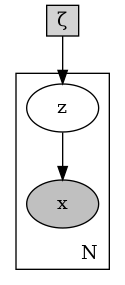
\includegraphics[width=\textwidth]{../plots/vae_p.gv.png}
\caption{generative model ($p(x,z)$}
%\caption{blabla}
%\label{bla}
\end{subfigure}
%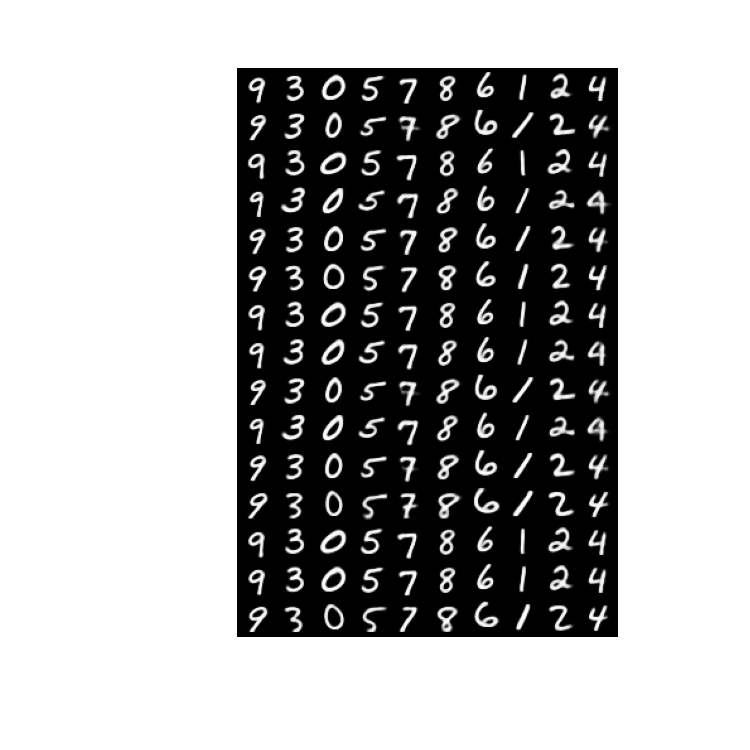
\includegraphics[width=0.4\linewidth]{images/model_mnist_10c_generation.png}
\begin{subfigure}[b]{0.2\textwidth}
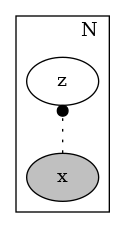
\includegraphics[width=\textwidth]{../plots/vae_q.gv.png}
\caption{inference model ($q(z|x)$)}
%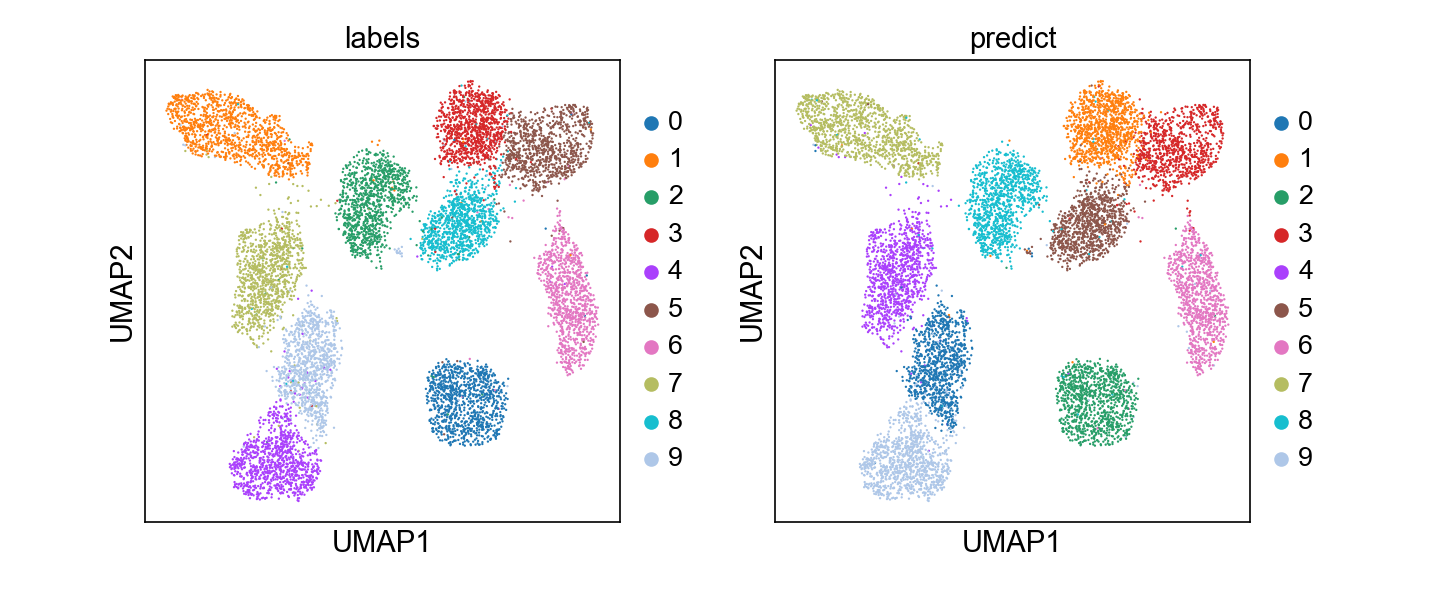
\includegraphics[width=0.4\linewidth]{images/model_mnist_10c_umap.png}
\end{subfigure}
\begin{subfigure}[b]{0.2\textwidth}
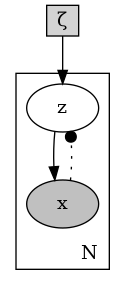
\includegraphics[width=\textwidth]{../plots/vae.gv.png}
\caption{the combined graphical model}
%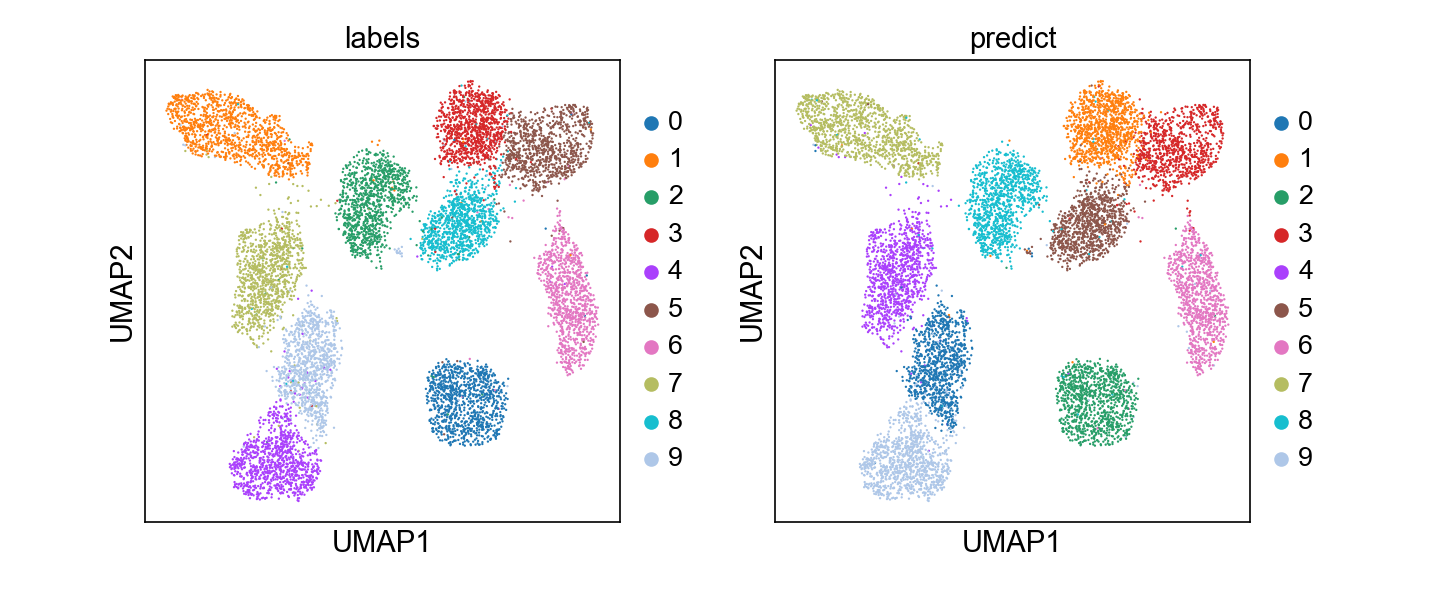
\includegraphics[width=0.4\linewidth]{images/model_mnist_10c_umap.png}
\end{subfigure}
\caption{VAE graphical model}
\label{fig:vae_model}
\end{figure}

\chapter{Gaussian mixture model VAEs}

Theoretical background and 
with some examples from publications and my own tests.


\begin{figure}
\centering
\begin{subfigure}[b]{0.4\textwidth}
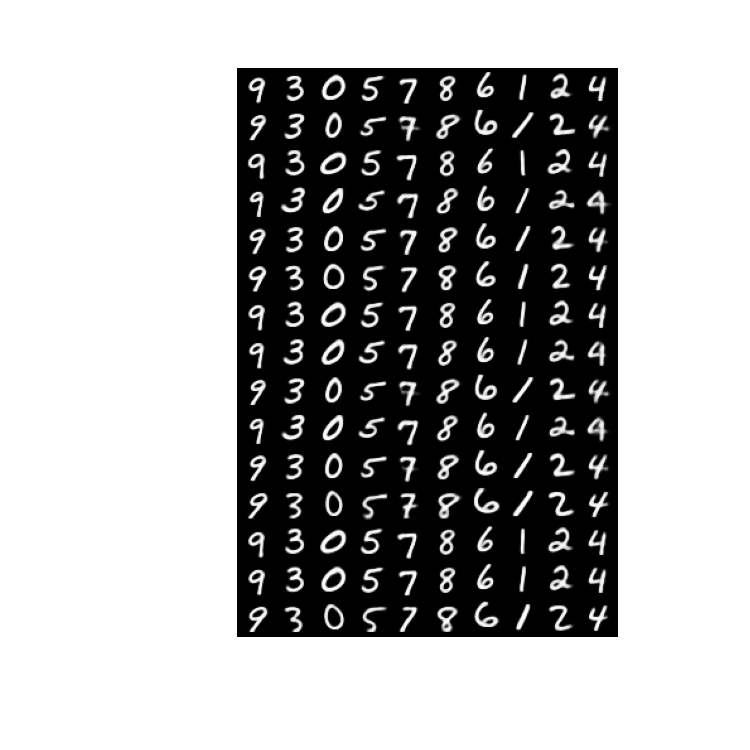
\includegraphics[width=\textwidth]{images/model_mnist_10c_generation.png}
\caption{}
%\caption{blabla}
%\label{bla}
\end{subfigure}
%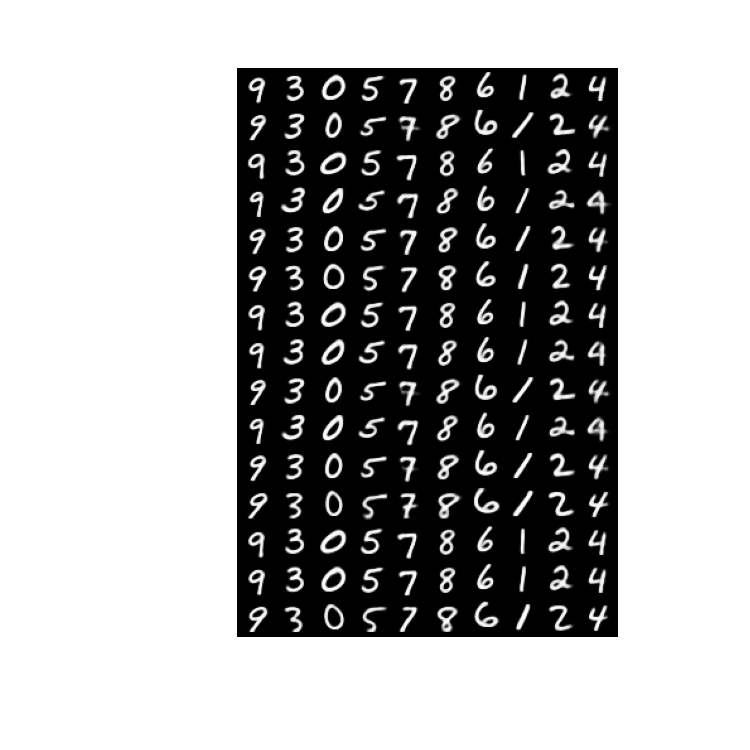
\includegraphics[width=0.4\linewidth]{images/model_mnist_10c_generation.png}
\begin{subfigure}[b]{0.4\textwidth}
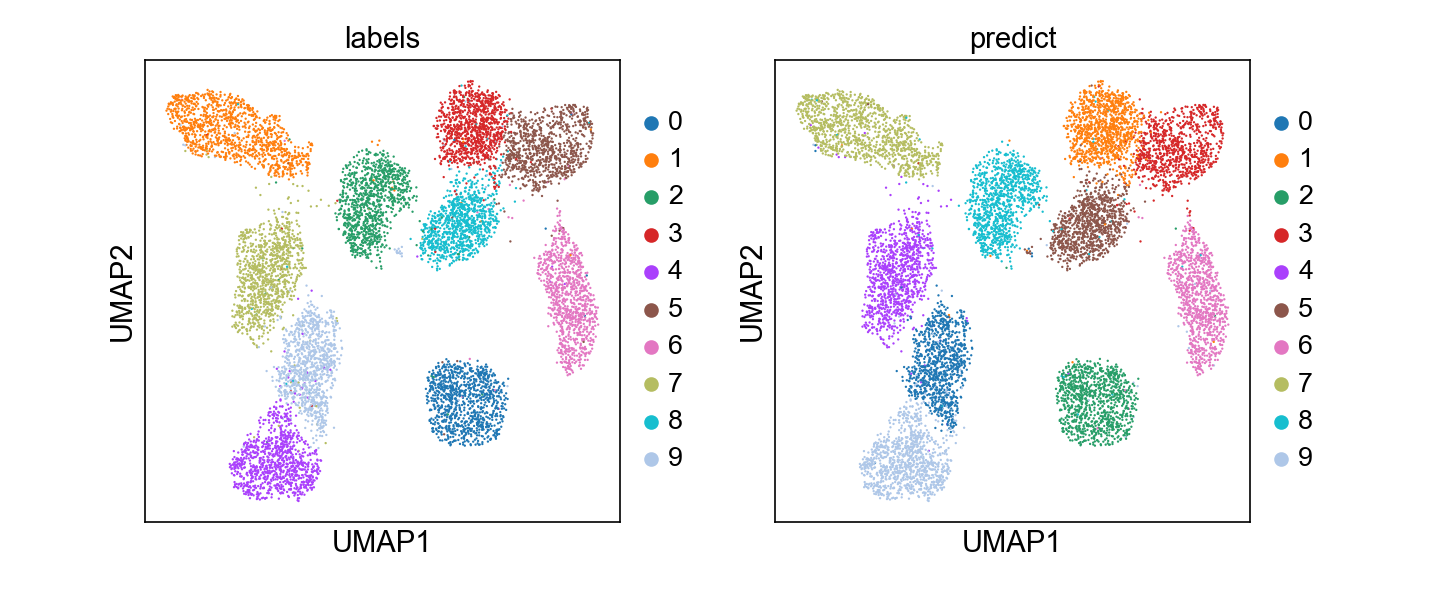
\includegraphics[width=\textwidth]{images/model_mnist_10c_umap.png}
\caption{}
%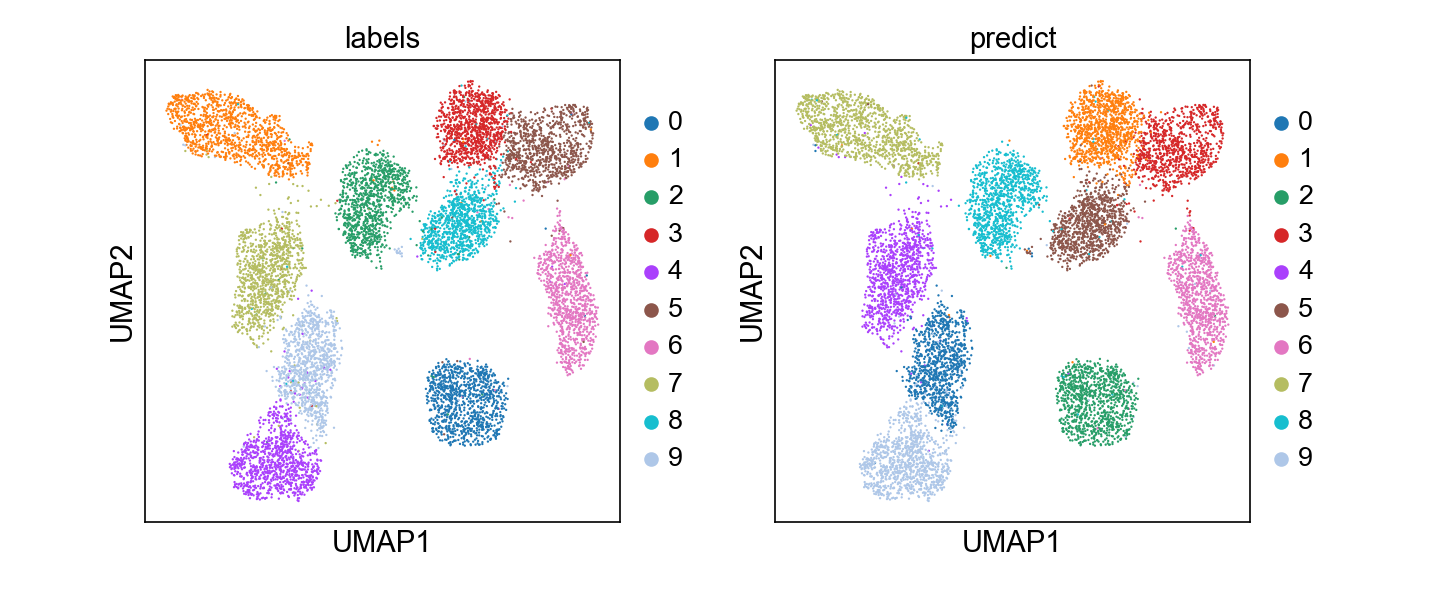
\includegraphics[width=0.4\linewidth]{images/model_mnist_10c_umap.png}
\end{subfigure}
\caption{a figure}
\label{fig:myfig}
\end{figure}

\subsection{Relation between AE and VAE}

\subsection{Conditional VAE}

\chapter{Experiments and results}
\section{Tests with MNIST and FMNIST}

\section{Tests with scRNAseq Data}
some words about (sc)RNAseq and published papers where 
AE and VAE models have been applied.
What we were hoping to achieve and compare with.

\chapter{Discussion, some remarks and conclusions}
punkt.
punkt.
punkt.





%\author{Yiftach Kolb}
%\date{Berlin, \today}
%\maketitle

%\section*{Intro Foo}
%\lipsum{1}
%\section{Bar}
%\lipsum{2}
%\appendix
%\section{Spam}
%\lipsum{3}

\printbibliography

\end{document}


